%%%%%%%%%%%%%%%%%%%%%%%%%%%%%%%%%%%%%%%%%
% Heavily modified by Razbit from the following template:
%
% Masters/Doctoral Thesis
% LaTeX Template
% Version 2.2 (21/11/15)
%
% This template has been downloaded from:
% http://www.LaTeXTemplates.com
%
% Version 2.x major modifications by:
% Vel (vel@latextemplates.com)
%
% This template is based on a template by:
% Steve Gunn (http://users.ecs.soton.ac.uk/srg/softwaretools/document/templates/)
% Sunil Patel (http://www.sunilpatel.co.uk/thesis-template/)
%
% Template license:
% CC BY-NC-SA 3.0 (http://creativecommons.org/licenses/by-nc-sa/3.0/)
%
%%%%%%%%%%%%%%%%%%%%%%%%%%%%%%%%%%%%%%%%%

%----------------------------------------------------------------------------------------
%	PACKAGES AND OTHER DOCUMENT CONFIGURATIONS
%----------------------------------------------------------------------------------------

\documentclass[
11pt, % The default document font size, options: 10pt, 11pt, 12pt
%oneside, % Two side (alternating margins) for binding by default, uncomment to switch to one side
english,
singlespacing, % Single line spacing, alternatives: onehalfspacing or doublespacing
%draft, % Uncomment to enable draft mode (no pictures, no links, overfull hboxes indicated)
%nolistspacing, % Uncomment this to set spacing in lists to single
%liststotoc, % Uncomment to add the list of figures/tables/etc to the table of contents
%toctotoc, % Uncomment to add the main table of contents to the table of contents
parskip, % Uncomment to add space between paragraphs
nohyperref, % Uncomment to not load the hyperref package
headsepline, % Uncomment to get a line under the header
]{class} % The class file specifying the document structure

\usepackage[utf8]{inputenc} % Required for inputting international characters
\usepackage[T1]{fontenc} % Output font encoding for international characters

\usepackage{palatino} % Use the Palatino font by default

\usepackage{pageslts}
\usepackage[titletoc]{appendix}

\usepackage{minted}
\renewcommand\listingscaption{Listaus}

\usepackage{etoolbox}
\AtBeginEnvironment{minted}{\singlespacing%
    \fontsize{10}{10}\selectfont}

\usepackage{graphicx}

\usepackage[backend=bibtex,style=authortitle,natbib=true]{biblatex}
\addbibresource{bibliography.bib} % The filename of the bibliography
\usepackage[autostyle=true]{csquotes} % Generate language-dependent quotes in the bibliography

%\pretolerance=10000
\tolerance=2000
\emergencystretch=10pt

%----------------------------------------------------------------------------------------
%	MARGIN SETTINGS
%----------------------------------------------------------------------------------------

\geometry{
	paper=a4paper, % Change to letterpaper for US letter
	inner=2.5cm, % Inner margin
	outer=3.8cm, % Outer margin
	bindingoffset=2cm, % Binding offset
	top=1.5cm, % Top margin
	bottom=1.5cm, % Bottom margin
	%showframe,% show how the type block is set on the page
}

%----------------------------------------------------------------------------------------
%	THESIS INFORMATION
%----------------------------------------------------------------------------------------

\thesistitle{UNIX-tyylinen käyttöjärjestelmäydin sekä ISO/IEC 9899:1999 ja POSIX.1-2008 -standardien mukainen C-kirjasto: RazOS} % \ttitle

\author{Pesonen, Eetu \& Rastas, Iiro} % \authorname
\webpage{http://github.com/razbit/razos} % \webpage
\keywords{Operating System, UNIX, POSIX, Programming} % \keywordnames
\newcommand\keywordnamesfi{Käyttöjärjestelmä, UNIX, POSIX, Ohjelmointi}
\university{Kerttulin Lukio} %  \univname
\department{ICT -linja} %  \deptname
\newcommand\nappendices{1} % Number of appendices. \nappendices

\abbrevnaming{Käytetyt merkinnät ja lyhenteet}

\begin{document}

\frontmatter % Use roman page numbering style (i, ii, iii, iv...) for the pre-content pages

\pagestyle{plain} % Default to the plain heading style until the thesis style is called for the body content

% For setting the chapter titles
\makeatletter
\def\@makechapterhead#1{
  \vspace*{10pt}
  {
    \reset@font\huge\bfseries
    \huge \thechapter{} \quad #1
    \par\nobreak
    \vskip 10pt
  }
}

\def\@makeschapterhead#1{%
  \vspace*{10pt}
  {
    \reset@font\huge\bfseries
    \huge #1
    \par\nobreak
    \vskip 10pt
  }
}


%----------------------------------------------------------------------------------------
%	TITLE PAGE
%----------------------------------------------------------------------------------------

\begin{titlepage}
\begin{center}

\textsc{\LARGE \univname}\\[1.5cm] % University name
\textsc{\Large ICT-linjan päättötyö}\\[0.5cm] % Thesis type

\doublespacing
{\huge \bf{\ttitle}}\\[0.4cm] % Thesis title
\singlespacing

Eetu Pesonen ja Iiro Rastas \\[0.4cm]

\deptname\\[2cm] % Research group name and department name

{\large \today}\\[4cm] % Date

\vfill
\end{center}
\end{titlepage}


%----------------------------------------------------------------------------------------
%	ABSTRACT PAGE
%----------------------------------------------------------------------------------------

\begin{abstract}
\addchaptertocentry{Tiivistelmä} % Add the abstract to the table of contents

\noindent
\MakeUppercase{\bf{\ttitle}}\\[0.4cm]
\authorname \\
\univname \\
\deptname \\
\today \\
Sivumäärä: \pageref{LastPage} (\lastpageref{LastPages})\\
Liitteitä: \nappendices \\
Asiasanat: \keywordnamesfi \\
\HRule

Käyttöjärjestelmät ovat monimutkaisia kokonaisuuksia. Työn tarkoitus on selventää käyttöjärjestelmän toimintaa ja toteutusta. Työssä kuvataan UNIX-tyylisen käyttöjärjestelmän teknistä toteutusta erityisesti prosessien, niiden hallinnan ja ajanjaon, muistinhallinnan sekä käyttäjän käytettävissä olevien rajapintojen kannalta. Teknisen toteutuksen kuvausta varten laadittiin UNIX-tyylinen käyttöjärjestelmä, RazOS. Toteutuksen kuvaukseen käytetään apuna lähdekoodia sekä teknisiä yksityiskohtia  selventäviä kaavioita.

\par

RazOS ohjelmoitiin C ja Assembly -ohjelmointikielillä, jotka ovat perinteisiä ohjelmointikieliä käyttöjärjestelmän ohjelmointiin. Alunperin C kehitettiin UNIX-käyttöjärjestelmän kehittämistä varten, joten se on erityisen sopiva ohjelmointikieli työn tarkoituksen kannalta. Alustaksi valittiin laajalti käytössä oleva Intelin x86 -arkkitehtuuri, koska yleisyytensä takia sille on helpompi laatia käyttöjärjestelmä kuin esimerkiksi ARM -arkkitehtuureille. Toinen syy x86:n valintaan oli sen ikä; sitä on käytetty lähes UNIXin alkuajoista asti, aina vuodesta 1978.

\par

Ohjelmointityön tuloksena saatiin aikaiseksi käyttöjärjestelmä, joka tukee osittain POSIX ja C99 -standardien mukaista C-kirjastoa. Sille tehtiin muutama ohjelma sekä komentotulkki, Rash. RazOSin kehitystyö jatkuu edelleen, ja tavoitteena on täysin standardien mukainen, UNIX-tyylinen käyttöjärjestelmä.

\end{abstract}

\clearpage

\begin{abstract}
\addchaptertocentry{Abstract} % Add the abstract to the table of contents

\noindent
\MakeUppercase{\bf{UNIX-like operating system kernel and ISO/IEC 9899:1999 and POSIX.1-2008 compliant C-library: RazOS}}\\[0.4cm]
\authorname \\
\univname \\
\deptname \\
\today \\
Number of pages: \pageref{LastPage} (\lastpageref{LastPages})\\
Appendices: \nappendices \\
Keywords: \keywordnames \\
\HRule

Operating systems are complex entities. The purpose of this work is to examine the workings and the implementation of an operating system. In this work we describe the technical implementation of a UNIX-like operating system, drawing particular attention to processes, their control and time-sharing, as well as to memory management and the interfaces available to the user. To illustrate the technical implementation, we have developed a UNIX-like operating system, RazOS. We use source code and figures of technical details to help illustrate this implementation.

\par

RazOS was programmed in traditional system programming languages, namely C and Assembly. C was originally created for the development of the UNIX operating system, so it is particularly suitable for work of this nature. We chose the widely used Intel x86 architecture as our target platform, since its prevalence makes it easier to develop an operating system to than some other architectures, such as ARM. The second reason for choosing x86 was its age; it has been in use since the infancy of UNIX, ever since 1978.

\par

Our development work has resulted in an operating system that partially supports the C library defined by the POSIX and C99 standards. We have developed some programs, as well as a shell, Rash. RazOS is actively developed, and our goal is a completely standards-compliant, UNIX-like operating system.

\end{abstract}


%----------------------------------------------------------------------------------------
%	LIST OF CONTENTS/FIGURES/TABLES PAGES
%----------------------------------------------------------------------------------------
\renewcommand{\contentsname}{Sisällysluettelo}
\tableofcontents % Prints the main table of contents


%----------------------------------------------------------------------------------------
%	ABBREVIATIONS
%----------------------------------------------------------------------------------------

\begin{abbreviations}{ll} % Include a list of abbreviations (a table of two columns)

\textbf{API} & \textbf{A}pplication \textbf{P}rogramming \textbf{I}nterface, ohjelmointirajapinta\\
\textbf{0x} & Etuliite heksadesimaaleille\\

\end{abbreviations}


%----------------------------------------------------------------------------------------
%	THESIS CONTENT - CHAPTERS
%----------------------------------------------------------------------------------------

\mainmatter % Begin numeric (1,2,3...) page numbering

\pagestyle{thesis} % Return the page headers back to the "thesis" style

% Include the chapters of the thesis as separate files from the Chapters folder
% Uncomment the lines as you write the chapters

\chapter{Johdanto}
\label{Johdanto}

Käyttöjärjestelmiä on useita, joista tunnetuimpia ovat Microsoft Windows, Applen Mac OS X sekä erinäiset Linux-versiot. Linux ja Mac OS X pohjautuvat teknisesti 1970-luvulla kehitettyyn UNIX-käyttöjärjestelmään, jota kehittivät Bell Labs -tutkimuslaitoksessa Dennis Richie ja Ken Thompson. Tässä työssä tarkastellaan käyttöjärjestelmän tehtäviä ja teknistä toteutusta UNIXin näkökulmasta tämän työn ohessa kehitetyn UNIX-tyylisen käyttöjärjestelmän, RazOSin, avulla.

\section{Käyttöjärjestelmän tehtävät}
Käyttöjärjestelmä on ohjelmisto, joka mahdollistaa muiden ohjelmien toiminnan hallinnoimalla tietokoneen resursseja, kuten muistia. Se antaa ohjelmien käyttöön yhtenäisen rajapinnan, API:n, joka on riippumaton alustasta. Rajapintaan kuuluu monia järjestelmäkutsuja, jotka toimivat erinäisten abstrahointien, kuten tiedostojärjestelmän ja virtuaalimuistin, kanssa.

\par

UNIX-maailmassa The Open Groupin ja IEEE Computer Societyn julkaisema POSIX-standardi määrittelee järjestelmäkutsuja ja laajentaa niiden avulla International Organization for Standardizationin ja International Electrotechnical Commissionin standardisoimaa C-kirjastoa. Standardisoidun C-kirjaston avulla ohjelmoijien on mahdollista kehittää ohjelmia, jotka toimivat kaikissa standardien mukaisissa käyttöjärjestelmissä, laitteistosta riippumatta.

\par

Käyttöjärjestelmä myös pitää huolta käyttäjän ja ohjelmien turvallisuudesta. Se esimerkiksi tarkistaa, onko käyttäjällä ja/tai ohjelmalla oikeus käyttää pyytämäänsä tiedostoa, ja suojelee muiden ohjelmien muistialueita virtuaalimuistinhallinan keinoin, etteivät ohjelmat käytä muistia, johon niillä ei ole lupaa koskea.

\par

Virheidenhallinta ja niistä selviäminen ovat myös käyttöjärjestelmän tehtäviä. UNIXeissa virheidenhallinta on tavallisesti hoidettu \textit{signaaleilla}, joita käyttöjärjestelmä antaa C-kirjastolle virheen sattuessa. Kirjasto hoitaa yleensä virheet itse, usein lopettamalla ohjelman suorituksen. Käyttäjä voi myös itse määrittää signaaleille käsittelyfunktion ISO-standardiin kuuluvalla \texttt{signal()} -funktiolla.
\chapter{Käyttöjärjestelmäydin}

\label{kernel}

\section{Yleistä}

Perinteisesti käyttöjärjestelmäytimet, kernelit, jaetaan monoliittisiin- ja mikroytimiin. Monoliittinen ydin sisältää kaikki ytimen toiminnot yhdessä osoiteavaruudessa, yhdessä kokonaisuudessa. Se on usein tehokkaampi ja helpompi kehittää kuin mikroydin, joka koostuu monesta osasta. Mikroytimeen perustuva käyttöjärjestelmä koostuu \textit{moduuleista}, joita pelkistetty \textit{mikroydin} ohjaa. Moduulit ovat usein käyttäjätilassa, englanniksi userspace, ydintilan (kernel space) sijaan. Koostuessaan useasta moduulista kokonaisuus on usein vakaampi kuin monoliittinen ydin, mutta hitaampi ja monimutkaisempi. UNIX-johdannaiset, kuten Linux, ovat yleensä monoliittisia.

\section{Käynnistys}

X86-tietokoneen käynnistyessä prosessori alkaa suorittaa koodia BIOSin ROM -muistista. BIOSin avulla etsitään ja otetaan käyttöön muisti ja kaikki laitteet ja saatetaan laitteisto sellaiseen tilaan, että ohjaus voidaan siirtää käynnistyslataajalle (bootloader) ja edelleen käyttöjärjestelmän ytimelle. Käynnistyslataajan toimintaan ei tässä tutustuta tarkemmin.

\subsection{Ytimen ensimmäiset askeleet}
Käynnistyslataaja siirtää ohjauksen ytimelle, eli paremmin sanottuna siirtää prosessorin suorittamaan ytimen koodia ladattuaan sen massamuistista RAM-muistiin. RazOSin tapauksessa prosessori siirtyy suorittamaan koodia osoitteesta 0x100000, eli yhden megatavun kohdalta muistin alusta laskien. Aluksi luodaan ja alustetaan pino, stack, otetaan käyttöön liukulaskentaprosessori, FPU, ja lopuksi siirrytään suorittamaan C-koodia (listaus 1).

\par

Siirryttyään C-koodin puolelle, alkaa prosessori suorittaa kmain()-funktiota. Sen avulla alustetaan laitteistoa ja otetaan käyttöön virtuaalimuisti. Lopuksi siirrytään käyttäjätilaan.

\begin{listing}[H]
\begin{minted}[]{nasm}
start:
    mov esp, stack_end   ; Luo ja alusta pino eli stack
    push dword 0
    push dword 0
    mov ebp, esp

    ;; Anna pinon alku ja multiboot-tiedot kmain():lle
    push esp
    push ebx

    fninit               ; Ota kayttoon FPU
    mov eax, cr0
    or eax, 1 << 5
    mov cr0, eax

    cli                  ; Poista kaytosta keskeytykset
    call kmain           ; Siirry suorittamaan C-koodia
\end{minted}
\caption{Käynnistyskoodia; razos/kernel/src/boot.s}
\label{lst:boot}
\end{listing}

\section{Virtuaalimuisti ja muistinhallinta}
Käynnistyksen aikana prosessori on ns. \textit{real mode}-tilassa, eli se käyttäytyy kuin 8086. Muistia ei ole käytettävissä kuin yksi megatavu, koska muistiosoitteet ovat 20-bittisiä. Käynnistyslataaja, tässä tapauksessa GNU GRUB, asettaa prosessorin 80386:n mukaiseen \textit{protected mode}-tilaan, jossa mukaan tulee uusia ominaisuuksia, tärkeimpinä virtuaalimuisti ja sivutus (paging). Muistiosoitteet kasvavat 32-bittisiksi, jolloin suurin mahdollinen määrä muistia on neljä gigatavua. Tietokoneessa ei kuitenkaan aina ole neljää gigatavua muistia, mutta koko osoiteavaruus on silti käytetävissä \textit{virtuaalisuutensa} takia. Fyysinen muisti on jaettu paloiksi, sivuiksi, ja virtuaaliosoiteavaruuden käytössä olevat muistialueet on ``mapattu'' tiettyihin sivuihin. Virtuaalimuisti mahdollistaa sen, että prosessorin osoiteavaruuteen voidaan liittää muutakin kuin vain RAM-muistia eli käyttömuistia. Esimerkiksi laitteita, kuten näytönohjain, voidaan mapata joihinkin muistiosoitteisiin, jolloin niihin osoitteisiin kirjoitettaessa tieto kulkeekin näytönohjaimelle eikä RAM-muistiin.

\par

Toinen virtuaalimuistin etu on se, että osoiteavaruuden kirjanpito voidaan tehä prosessikohtaiseksi. Tällöin jokainen prosessi voi olla täysin tietämätön muista prosesseista, eikä sen tarvitse tietää mihin kohtaan \textit{fyysistä} musitia se on ladattu, koska jokaisen prosessin osoiteavaruus alkaa nollasta ja päättyy neljään gigatavuun, osoitteeseen 0xFFFFFFFF. Muistia on myös helpompi suojella, kun käyttöjärjestelmä saa tarkistettua jokaisen luku- ja kirjoitusoperaation ja voi määrittää sivukohtaisesti mitä prosessi saa muistilla tehdä. Fyysisen muistin sivusta käytetään usein englanninkielistä nimitystä \textit{frame}, ja virtuaalisen muistin sivusta nimitystä \textit{page}.

\begin{figure}[H]
\centering
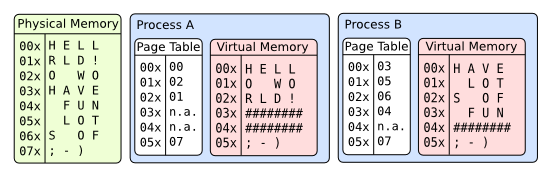
\includegraphics[width=\textwidth]{../figures/virtual_memory.png}
\caption{Virtuaalimuisti havainnollistettuna}
\label{fig:virtual_memory}
\end{figure}

\subsection{Virtuaalimuistin hallinta}

Muistinhallinnan perustehtäviä on varata ja vapauttaa muistia ohjelmien tarpeen mukaan, mahdollisimman tehokkaasti.

\subsubsection{Sivutus}

X86-arkkitehtuuri toteuttaa virtuaalimuistin sivutuksella, kun prosessori on protected mode -tilassa. Sivutuksen kirjanpito on kolmetasoinen:
\begin{figure}[H]
\centering
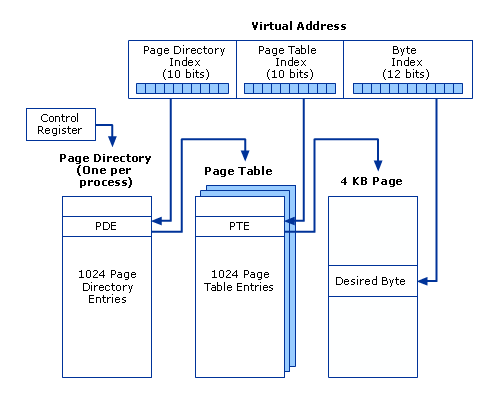
\includegraphics[width=\textwidth]{../figures/paging.png}
\caption{Sivutuksen kirjanpito}
\label{fig:paging}
\end{figure}

Prosessorin ohjausrekisteri CR3 sisältää kulloinkin käytössä olevan \textit{page directoryn} fyysisen muistiosoitteen. Page directory sisältää 1024 \textit{page directory entryä} (PDE), joiden \textit{flageilla} voi määrätä ominaisuuksia kutakin entryä vastaavaan \textit{page tableen}, joissa on jokaisessa puolestaan 1024 \textit{page table entryä} (PTE). PTE sisältää yhden neljän kilotavun sivun fyysisen osoitteen ja joitakin flageja, joiden avulla määritellään, onko esimerkiksi sivulle kirjoittaminen sallittua.

\par

Virtuaalinen muistiosoite on 32 bittiä pitkä. Sen 10 suurinta bittiä (bitit 31..21) ovat indeksi page directoryyn, eli kertovat mikä page table sisältää kyseisen sivun. Seuraavat kymmenen bittiä puolestaan ovat indeksi page tableen, eli kertovat mikä sivu on kyseessä. Loput 12 bittiä ovat halutun tavun etäisyys sivun alusta. RazOSissa page directory entryä kuvataan structilla pg\_dir\_entry\_t, ja page table entryä structilla page\_t.

\begin{listing}[H]
\begin{minted}[]{c}
struct page_t
{
	uint32_t present : 1;    /* Page present in memory */
	uint32_t rw : 1;         /* Page writable */
	uint32_t user : 1;       /* User-accessible */
	uint32_t wt_caching : 1; /* Write-through caching */
	uint32_t nocache : 1;    /* Caching disabled */
	uint32_t accessed : 1;   /* Has been accessed */
	uint32_t dirty : 1;      /* Has been written to */
	uint32_t zero : 1;       /* Always zero */
	uint32_t global : 1;     /* Global: do not flush in TLB flush */
	uint32_t avail : 3;      /* Bits not used by CPU */
	uint32_t frame : 20;     /* Physical address of the frame */
};

struct pg_dir_entry_t
{
	uint32_t present : 1;    /* Page present in memory */
	uint32_t rw : 1;         /* Page writable */
	uint32_t user : 1;       /* User-accessible */
	uint32_t wt_caching : 1; /* Write-through caching */
	uint32_t nocache : 1;    /* Caching disabled */
	uint32_t accessed : 1;   /* Has been accessed */
	uint32_t zero : 1;       /* Always zero */
	uint32_t size : 1;       /* 0 = 4K, 1 = 4M pages */
	uint32_t global : 1;     /* Global: do not flush in TLB flush */
	uint32_t avail : 3;      /* Bits not used by CPU */
	uint32_t table : 20;     /* Physical address of the page table */
};
\end{minted}
\caption{Sivutuksen tietorakenteita RazOSissa}
\label{lst:paging_structs}
\end{listing}

\par

Kun tarvitaan lisää muistia, aloitetaan etsimällä vapaa fyysinen sivu. RazOSissa sen hoitaa \texttt{frame\_alloc()}, joka palauttaa sivun fyysisen osoitteen. Tämän jälkeen sivu mapataan haluttuun virtuaaliosoitteeseen funktion \texttt{page\_map()} avulla. Se asettaa myös halutut flagit, esimerkiksi onko sivu vain ytimen käytössä vai saako käyttäjätason ohjelmatkin käyttää sitä. Tämän jälkeen tehdään ``TLB Flush'', eli tyhjennetään prosessorin välimuistista kyseistä virtuaaliosoitetta vastaava fyysinen osoite, jotta prosessori laskee uuden, jolloin muistioperaatiot tapahtuvat oikeassa, uudessa kohdassa fyysistä muistia. Muistin vapauttaminen toimii samalla tavalla, ensin poistetaan mappaus kyseisestä virtuaaliosoitteesta, merkitään sivu poissaolevaksi ja lopuksi merkitään fyysinen sivu vapaaksi funktiolla \texttt{frame\_free()}.

\subsubsection{Muistin varaaminen}

Kun muistia halutaan käyttää, täytyy sitä varata. Muistia käytetään pääosin kolmella tavalla: on pino (stack), dynaaminen muistialue (heap) sekä ohjelmakoodille varattu, suoritettava alue. Yksittäiset muuttujat tallennetaan yleensä pinoon, ja esimerkiksi funktiota kutsuttaessa sen parametrit ja paluuosoite tallennetaan pinoon. Heappiä käytetään dynaamiseen varaukseen ja vapautukseen esimerkiksi suurten listojen kanssa. Pino on kooltaan hyvin pieni, kun heap puolestaan on todella suuri: RazOSissa pinon koko on 64 kilotavua, heapille on varattu virtuaaliosoitteita yli kolmen gigatavun edestä.

\par

Muistin varaaminen heapiltä tapahtuu C-standardin mukaan \texttt{malloc()}-perheen funktioilla. Malloc tarvitsee tosin heap-alueen toimiakseen, ja sen käsittelyyn, laajentamiseen ja pienentämiseen, on perinteisesti kaksi funktiota; \texttt{brk()} ja \texttt{sbrk()}, jotka POSIX ennen määritteli. Funktiot \texttt{brk()} ja \texttt{sbrk()} käyttävät funktiota \texttt{page\_map()} sivujen varaamiseen ja vapauttamiseen. Nykyään standardiin kuuluu niiden sijaan \texttt{mmap()}, mutta sen tarkastelu sivuutetaan. Malloc -implementaatioita on useita, joista ehkä tunnetuin on Doug Lean malloc, dlmalloc. Dlmalloc on melko joustava, ja siksi sitä käytetään paljon \parencite{dlmalloc}. Muitakin implementaatioita on tehty, joissakin on tarkoituksena säästää muistia ja toisissa prosessoriaikaa.

\par

RazOSin malloc, rmalloc, lainaa joitain dlmallocin ajatuksia, ja on hyvin yksinkertainen. Rmallocista on kaksi eri versiota; toinen ytimen käyttöön ja toinen käyttäjämaailman prosessien käyttöön. Käyttäjämaailman toimintaa tarkastellaan myöhemmin. Funktioiden ero on siinä, miten varattu muisti sijoitetaan osoiteavaruuteen: ytimelle on monissa tapauksissa tärkeää, että osoitteet ovat esimerkiksi jaollisia yhden sivun koolla, neljällä kilotavulla. Käyttäjämaailmassa ei tällaista rajoitusta ole, joten käyttäjämaailman rmalloc on hieman yksinkertaisempi.

\begin{figure}[H]
\centering
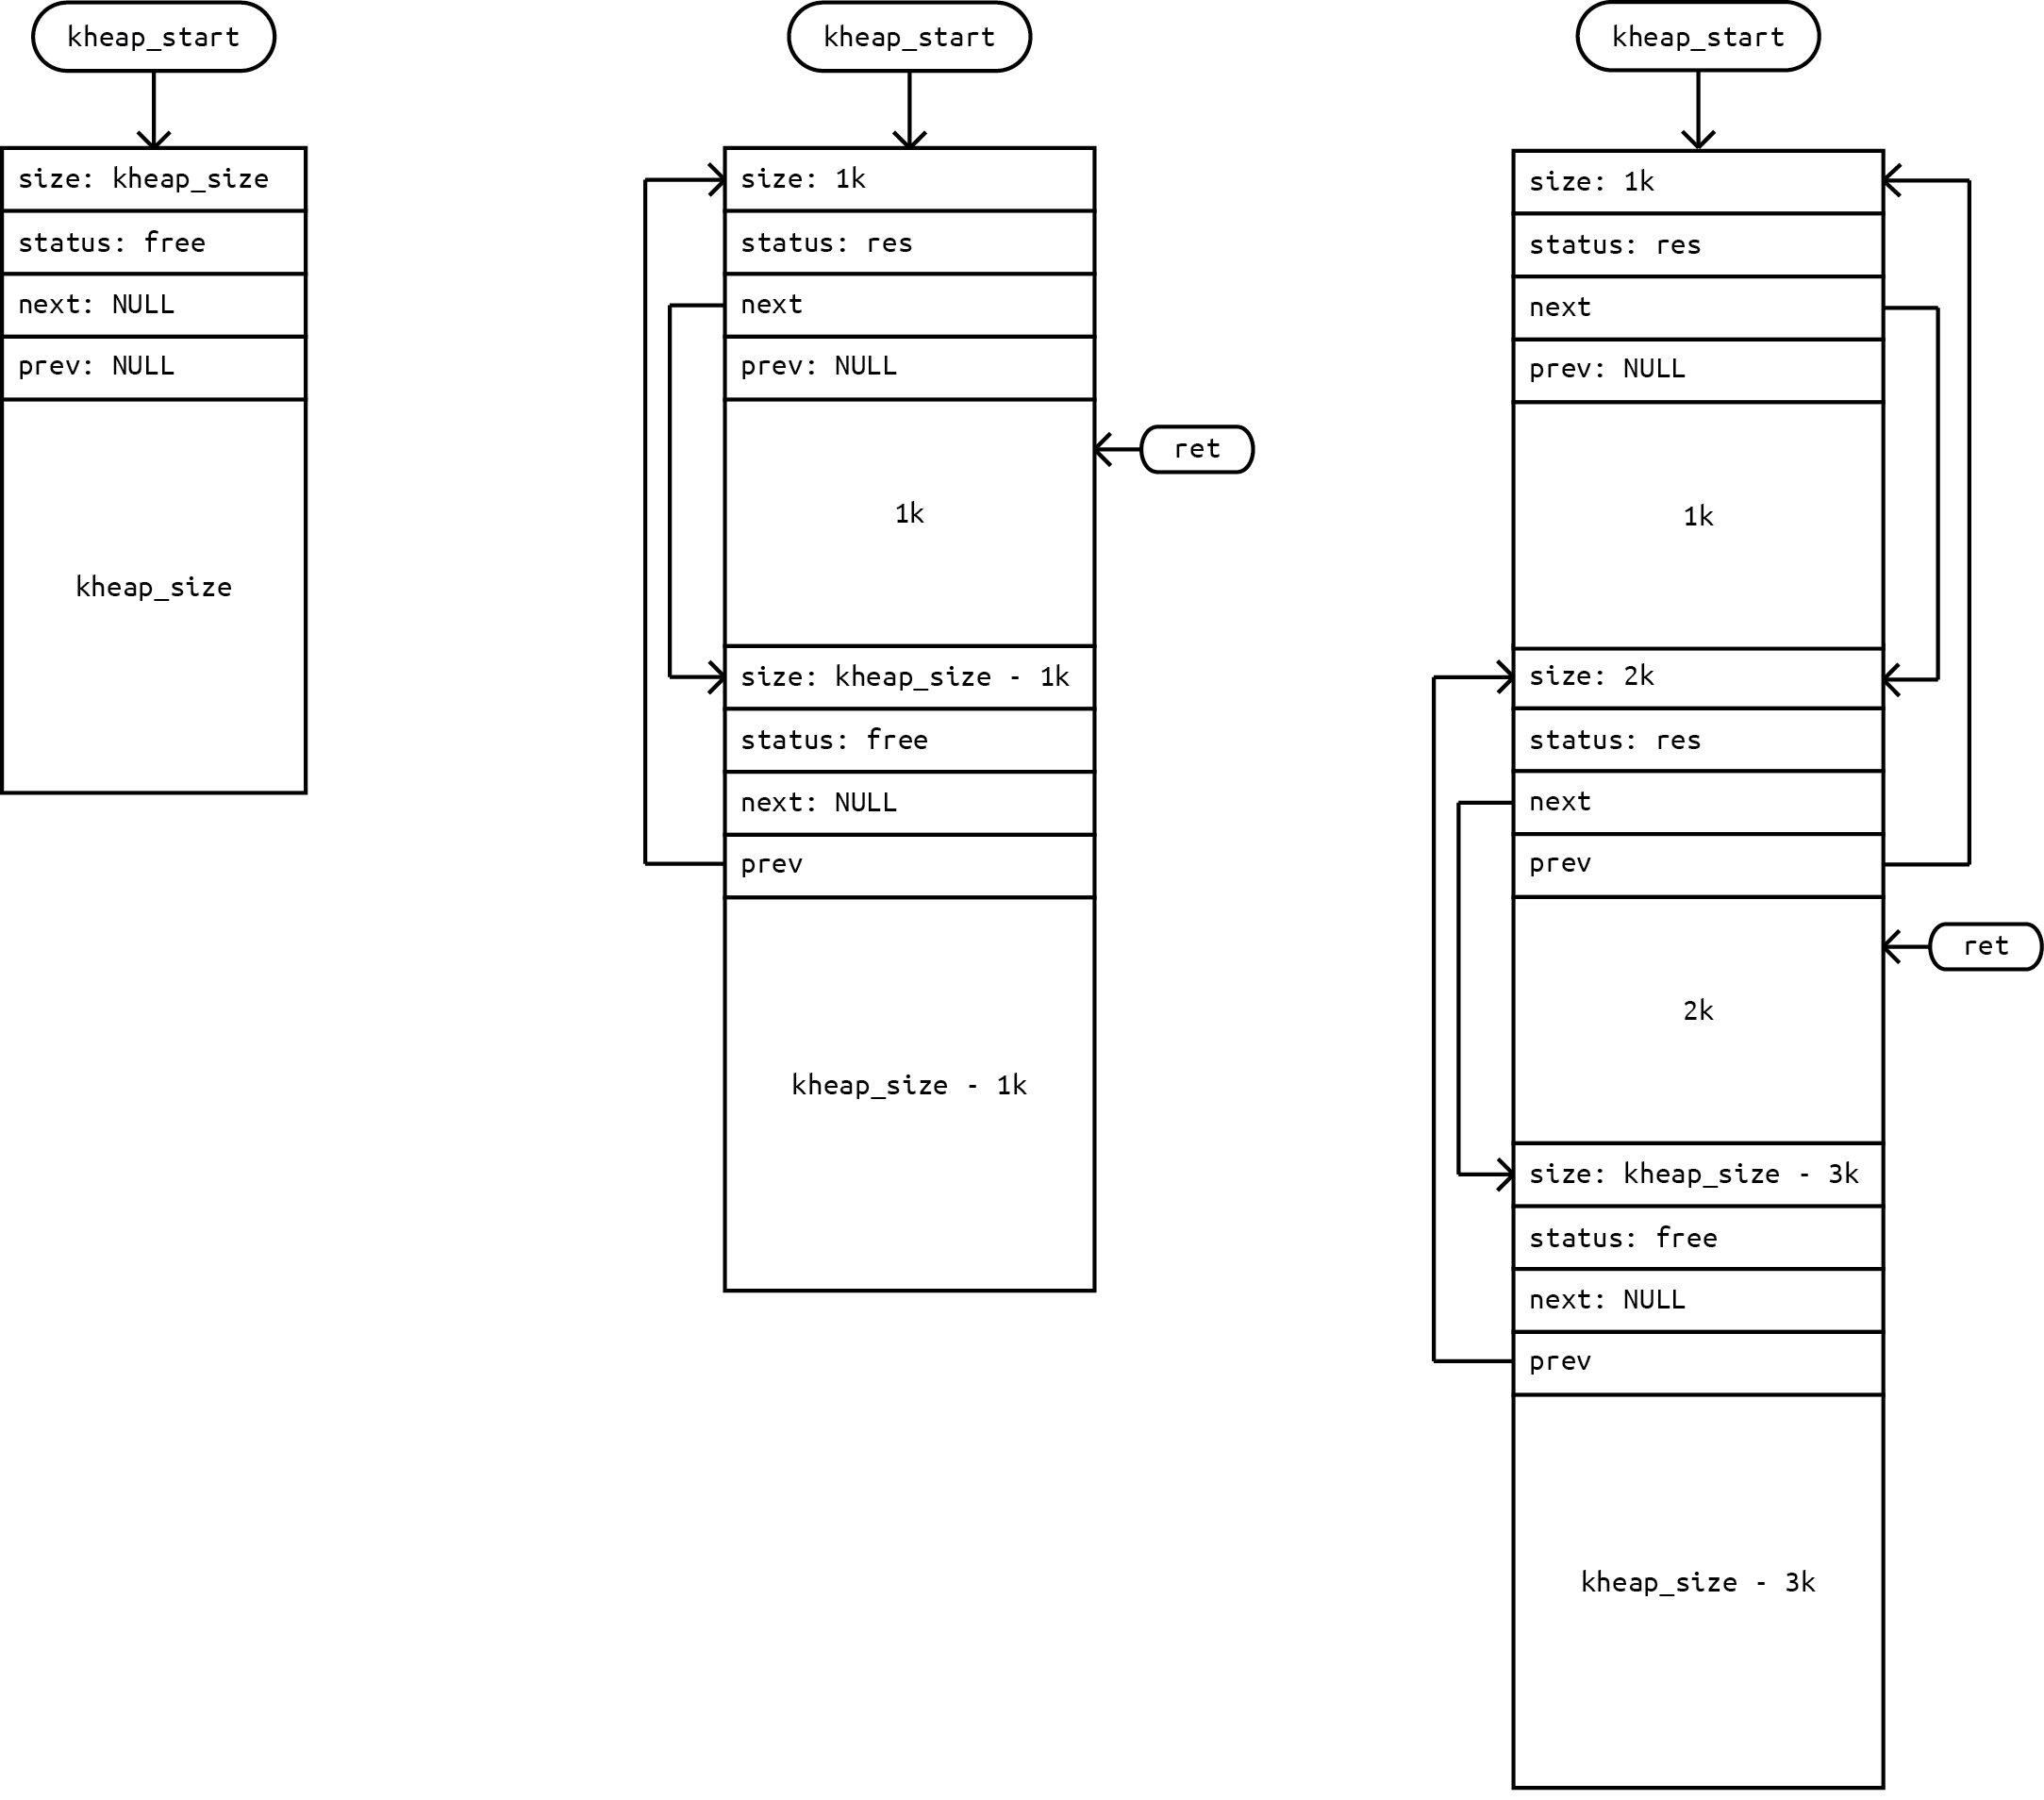
\includegraphics[width=\textwidth]{../figures/rmalloc.png}
\caption{Graafi rmallocin toiminnasta. Alkutilanne, yksi yhden kilotavun varaus ja viimeisessä toinen, kahden kilotavun varaus.}
\label{fig:rmalloc}
\end{figure}

\subsubsection{Muistin vapauttaminen}
Kun halutaan vapauttaa muistia heapiltä, käytetään perinteisesti funktiota \texttt{free()}. Se merkitsee mallocilla varatun muistin vapaaksi, yhdistää läheiset vapaat muistialueet (coalescing) ja mikäli mahdollista, pienetää heap-aluetta \texttt{sbrk()}:n avulla.

\begin{figure}[H]
\centering
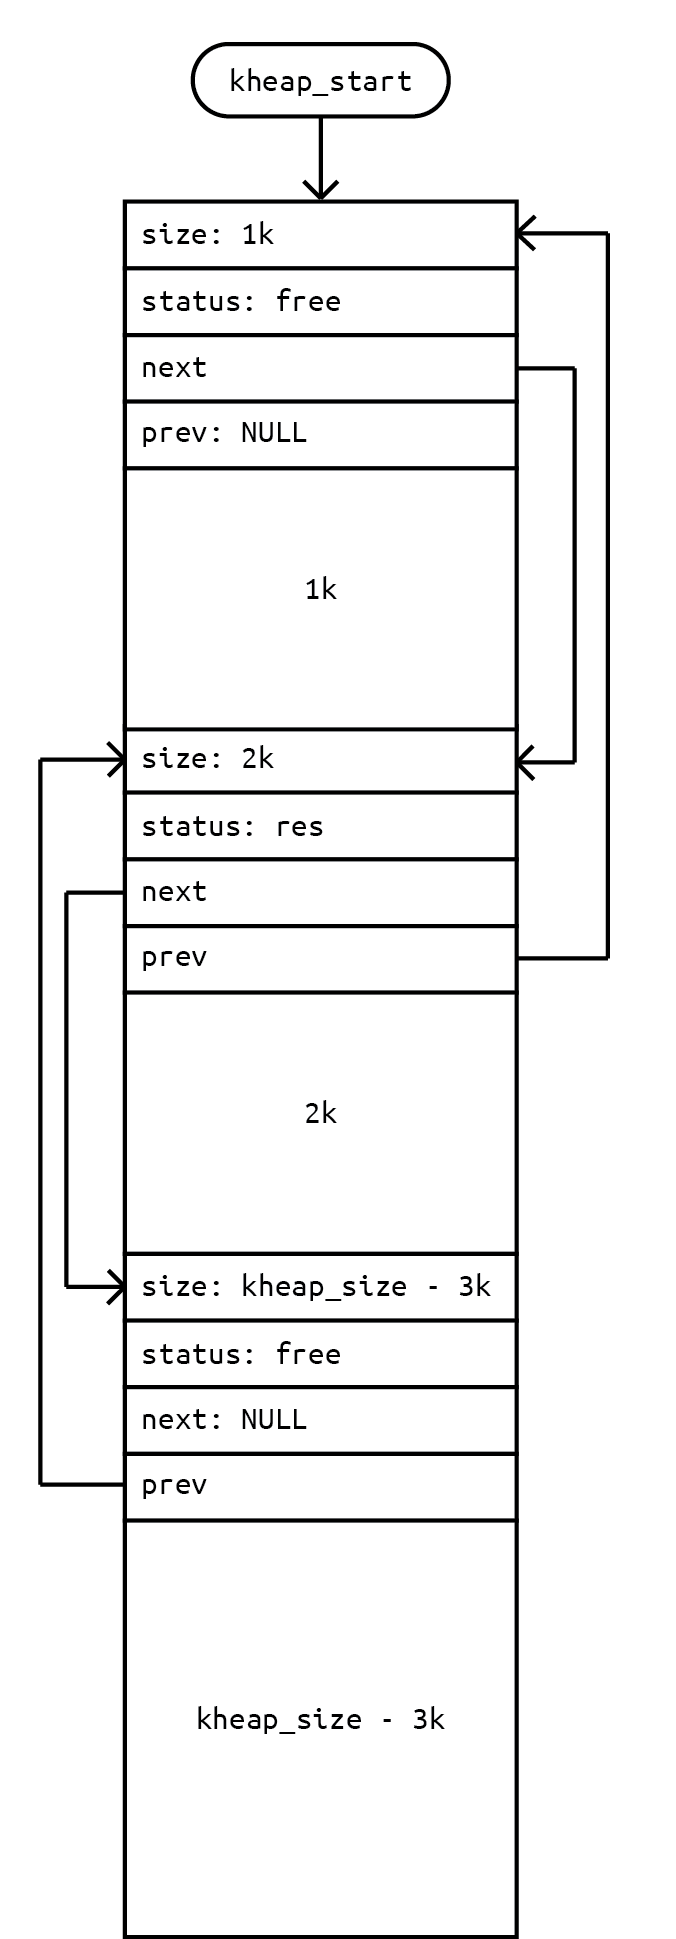
\includegraphics[]{../figures/rfree.png}
\caption{Kuvan \ref{fig:rmalloc} viimeisen tapauksen mukaisesta heapistä on vapautettu ensimmäinen, yhden kilotavun varaus.}
\label{fig:rfree}
\end{figure}

\section{Keskeytykset}

Keskeytys (interrupt) on joko laitteiston tai ohjelman aikaansaama signaali, joka keskeyttää prosessorin toiminnan. Keskeytyksen tullessa suoritin tallentaa tilansa pinoon, ja siirtyy suorittamaan keskeytyskäsittelijää (interrupt handler). Kun käsittelijän suoritus on saatu päätökseen, palauttaa prosessori tilansa pinosta ja jatkaa siitä, mihin jäi keskeytyksen tullessa. Keskeytyksiä käytetään yleensä siihen, että tietokone saa tiedon erinäisitä tapahtumista, kuten näppäimistön napin painalluksista tai ajastimen (PIT, programmable interrupt timer) laukeamisesta. Tällöin prosessorin ei tarvitse koko ajan tarkistaa, onko jotain tapahtunut, jolloin prosessoriaikaa säästyy.

\par

X86-arkkitehtuurilla keskeytyskäsittelijöiden sijainti on tallennettu IDT-taulukkoon (Interrupt Descriptor Table). Jokainen keskeytys on numeroitu, ja IDT:stä löytyy jokaista numeroa vastaavan käsittelijän osoite, johon prosessori hyppää keskeytyksen tullessa.

\subsection{Poikkeukset}

Poikkeukset (exception) ovat keskeytyksiä, joita prosessori itse aiheuttaa. Tyypillisiä poikkeus ovat nollalla jako ja sivutusvirhe (page fault). Niiden tullessa, on prosessori yrittänyt suorittaa jotain käskyä siinä onnistumatta.

\subsubsection {Sivutusvirhe}

Sivutusvirhe tulee, kun yritetään käyttää muistia, jota ei ole mapattu tai jota ei saa käyttää. Sivutusvirheen virhekoodi kertoo, mikä meni pieleen; eikö muistia oltu mapattu, eikö muistiin kirjoittaminen ollut sallittua tai eikö käyttäjätason ohjelma saanut siihen koskea. Virheen käsittelijä voi olla hyvinkin monimutkainen, sillä se voi yrittää korjata tilannetta. Esimerkiksi Linux tukee niin sanottua \textit{demand pagingiä}, jossa virtuaaliosoitetta ei mapata fyysiseen sivuun ennen ensimmäistä käyttöyritystä. Tällöin säästetään fyysistä muistia muiden prosessien käyttöön.

\par

Yksinkertaisimmillaan käsittelijä vain ilmoittaa ongelmasta ja lopettaa ongelman aiheuttaneen ohjelman suorituksen. Yleensä ongelma tosin pyritään korjaamaan, mutta se ei aina ole mahdollista. Silloin UNIX-variantit lähettävät \texttt{SIGSEGV} -signaalin, jolla prosessi lopetetaan. RazOS ei vielä tue signaaleja, joten RazOSin sivutusvirhekäsittelijä vain lopettaa suorituksen.

\subsection{Laitteistokeskeytykset}

Laitteistokeskeytykset (Interrupt request, IRQ) aiheutuvat laitteiston toiminnasta. Esimerkiksi näppäimistön nappia painettaessa lähtee prosessorille tieto keskeytyksestä numero 33, jolloin prosessori etsii IDT:stä oikean käsittelijän ja hyppää siihen. Aluksi tallennetaan prosessorin tila, kerrotaan näppäimistölle, että keskeytys on huomattu ja jatketaan keskeytyksen käsittelyä.

\begin{listing}[H]
\begin{minted}[]{nasm}
isr_33:
    pusha           ; Prosessorin tilan tallennus pinoon

    ;; Ilmoitetaan nappaimistolle keskeytyksen huomaamisesta
    push ax
    mov al, 0x20
    out 0xa0, al
    out 0x20, al
    pop ax

    call kb_handler ; Hypataan C-koodin puolelle
    popa            ; Palautetaan prosessorin tila
    iret            ; Jatketaan suoritusta siita, mihin jaatiin
\end{minted}
\caption{Näppäimistökeskeytyksen käsittely; razos/kernel/src/drivers/isr.s}
\label{lst:kb_isr}
\end{listing}

\section{Moniajo}

Moderni käyttöjärjestelmä kykenee moniajoon, eli sillä voi käyttää useampaa ohjelmaa samaan aikaan. Myös UNIX ja sen variantit kykenevät siihen, myös RazOS. Moniytiminen prosessori kykenee suorittamaan useaa prosessia samaan aikaan, mutta tässä tarkastellaan vain yksiytimisiä prosessoreita, joissa moniajo toteutetaan jakamalla prosessoriaika usean prosessin (säikeen, thread of execution) välillä. Oiva työkalu siihen on ajastimen aiheuttamat keskeytykset; ajastimen keskeytyskäsittelijä vaihtaa suoritettavan prosessin aina ajastimen lauetessa.

\subsection{Moniajo UNIX-varianteissa}

\subsubsection{fork-exec}

UNIX ja sen variantit, mukaan lukien RazOS, hoitavat moniajon ja uuden prosessin aloituksen niin sanotulla \textit{fork-exec} -menetelmällä. Siinä käytetään funktiota \texttt{fork()} kopioimaan jonkin prosessin (vanhempi, parent) osoiteavaruus, jolloin syntyy toinen, samaa koodia suorittava prosessi (lapsi, child). Lapsi jatkaa suoritusta samasta kohdasta vanhempansa kanssa, mutta sillä on oma kopionsa muistista käytössä, ja se siis työskentelee omassa osoiteavaruudessaan, jolloin sillä on oma \textit{page directory}. Tämän jälkeen voidaan kutsua jotain \texttt{exec}-perheen funktiota, RazOSissa \texttt{execve()} tai \texttt{execv()}, jolla vaihdetaan suoritettava koodi (process image), eli siirrytään suorittamaan eri ohjelmaa. Prosesseista käytetään UNIX-termiä \textit{task}. Kun lapsi on suoritettu loppuun, kutsutaan C-kirjaston funktiota \texttt{exit()}, joka siirtää suorituksen ytimelle. Ydin vapauttaa lapsen varaaman muistin ja ilmottaa sen vanhemmalle lapsen ``kuolleen'' ja kertoo sen palautusarvon. Tämän jälkeen kaikki jäänteet lapsesta siivotaan muistista, ja palataan suorittamaan muita prosesseja.

\par

RazOSissa jokaista prosessia kuvaa \texttt{struct task\_t}, joka sisältää kaiken oleellisen tiedon prosessista:

\begin{listing}[H]
\begin{minted}[]{c}
struct task_t
{
	uint8_t fpu_state[512];      /* Liukulukuprosessorin tila */
	uint32_t esp;                /* Pinon alku */
	uint32_t eip;                /* Suoritettavan kaskyn osoite */
	struct page_dir_t* page_dir;

	struct registers_t* syscall_regs; /* Prosessorin rekisterit */

	pid_t pid;                   /* Prosessin numero */
	pid_t ppid;                  /* Vanhemman numero */

	uint32_t state;
	uint32_t exit_status;        /* Palautusarvo */

	uint32_t children;           /* Lapsien maara */

	struct task_t* wait_queue;   /* ``Kuolleiden'' lasten lista */

	void* uheap_begin;           /* Kayttajapuolen heap-alueen alku */
	void* uheap_end;

	struct fildes_t files[OPEN_MAX]; /* Kaytossa olevat tiedostot */
	int* errno_loc;              /* errno-virhekoodin osoite */
};
\end{minted}
\caption{task\_t; razos/kernel/src/mm/task.h}
\label{lst:task_t}
\end{listing}

\par

Funktion \texttt{fork()} implementaatioon voi tutustua tiedostojen \texttt{razos/kernel/src/mm/task.c} ja \texttt{razos/kernel/src/mm/task.s} avulla.

\subsubsection{Ohjelman lataus}

Tietokoneohjelmia tehdään monessa muodossa. UNIX-maailmassa niistä yleisin on ELF (Executable and Linkable Format). ELF-tiedosto pitää sisällään ohjelmakoodin, etukäteen alustetut muuttujat (kuten merkkijonot) ja ohjeet käyttöjärjestelmälle siitä, miten tiedosto kuuluu ladata (virtuaali-) muistiin. Lataaja avaa tiedoston ja kopioi sen sisällön ohjeiden mukaan oikeisiin kohtiin osoiteavaruutta. Tämän jälkeen suoritus siirtyy uuden ohjelman alkuun.

\par

Ohjelman lataukseen käytetään jotain \texttt{exec()}-funktioista. Ne antavat ohjelmalle lisäksi argumentteja ja ympäristömuuttujia (environment variable). Funktio vapauttaa käyttäjän muistialueet, sulkee avoimet tiedostot ja vaihtaa ohjelmakoodin. RazOSissa \texttt{exec()}-funktioperheen kaikki funktiot perustuvat funktioon \texttt{execve()}. Sen lähdekoodi löytyy kansiosta \texttt{razos/kernel/src/loader/}.

\subsubsection{Prosessin vaihto}

Ajastimen lauetessa kutsutaan vuorontajaa (scheduler), joka valitsee seuraavan suoritettavan prosessin. Aluksi vuorontaja tallentaa vanhan prosessin tilan, RazOSissa \texttt{task\_t}:hen, jotta sen suoritukseen voidaan myöhemmin palata ongelmitta. Sen jälkeen valitaan uusi prosessi funktiolla \texttt{sched\_next()}, vaihdetaan osoiteavaruus eli kirjoitetaan \texttt{CR3}-ohjausrekisteriin uuden prosessin page directoryn osoite ja lopuksi palautetaan uuden prosessin tila \texttt{task\_t}:stä. Tämän jälkeen vuorontajan suoritus loppuu ja hypätään \texttt{task\_t}:stä otettuun suoritusosoitteeseen (rekisteri EIP, [Extended] Instruction Pointer), josta palataan usein käyttäjämaailmaan ja siellä jatketaan prosessin suoritusta seuraavaan ajastimen laukeamiseen asti.

\begin{listing}[H]
\begin{minted}[]{nasm}
sched_switch:
    ;; Tallenna vanhan prosessin tila
    pusha
    mov eax, [cur_task]
    fxsave task_fpu_state(eax)
    mov task_esp(eax), esp
    mov task_eip(eax), dword .return ; Osoite, josta suoritus jatkuu

    ;; Valitse uusi prosessi
    call sched_next
    mov [cur_task], eax

    ;; Hae page directoryn fyysinen osoite
    push dword task_page_dir(eax)
    call get_page_dir_phys
    add esp, 4

    ;; Lataa se CR3:een
    mov cr3, eax

    mov eax, [cur_task]

    ;; Palauta prosessin tila
    fxrstor task_fpu_state(eax)
    mov esp, task_esp(eax)
    jmp task_eip(eax)

.return:
    popa
    ret
\end{minted}
\caption{Vuorontajan assemblyllä kirjoitettu osa; razos/kernel/src/mm/task.s}
\label{lst:sched_switch}
\end{listing}

\par

Vuoronnusalgoritmeja on useita. Yleensä prosesseille voidaan määrittää prioriteetti, jonka mukaan määrätään mikä prosessi saa eniten suoritusaikaa. Yksinkertaisissa algoritmeissa ei priorisointia ole. Esimerkiksi RazOS käyttää nk. kiertovuorottelumenetelmää (round robin scheduling), jossa jokainen prosessi saa käyttää aikaa korkeintaan jonkin tietyn aikaviipaleen (time slice) verran. Tämän jälkeen prosessia vaihdetaan ja ajossa ollut prosessi laitetaan jonon viimeiseksi. Menetelmä on \textit{irrottava}, koska ydin voi määrätä milloin prosessin aikaviipale loppuu ja on vaihdettava prosessia. Irrottavan vuoronnuksen vastakohta on ei-irrottava vuoronnus, jossa prosessilta ei voida viedä vuoroa pois, vaan se luovuttaa sen itse. Sekin on usein mahdollista irrottavaa vuoronnusta käyttävissä järjestelmissä. Esimerkiksi RazOSissa prosessi antaa suoritusvuoronsa pois, jos se joutuu odottamaan esimerkiksi lukuoperaation valmistumista. Siihen käytetään funktiota \texttt{sched\_yield()}.

\section{Tiedostojen hallinta}

Yksi käyttöjärjestelmän tärkeistä osista on tiedostojen hallitseminen. Se on laaja kokonaisuus, jossa noustaan abstraktiotasolta toiselle, kunnes C-kirjaston yleiset metodit (tiedostossa \texttt{stdio.h}) ovat käytettävissä. POSIX tuo omia keinojaan, jotka ovat abstraktioltaan paljon alempana C-kirjastoa. Abstraktion tarkoituksena on, että ohjelmoija voi samalla tavalla käyttää mitä tahansa tiedostoksi ajateltavaa kokonaisuutta: kiintolevyllä olevaa tiedostoa, sarjaporttia tai vaikkapa USB-väylää. Abstraktiota kutsutaan virtuaalitiedostojärjestelmäksi (Virtual File System, VFS). RazOSissa VFS kuvaa tiedostoja ja niihin verrattavia kokonaisuuksia structeilla \texttt{vfs\_node\_t} ja \texttt{stat} ja käsittelee avoimia tiedostoja structin \texttt{fildes\_t} avulla.

\begin{listing}[H]
\begin{minted}[]{c}
struct vfs_node_t
{
	char name[64];      /* Tiedoston nimi */
	struct stat status;

    /* Kyseisen tiedostojarjestelman kasittelyfunktiot,
     * kuuluvat laitteen/tiedostojarjestelman ajuriin */
	read_t read;
	write_t write;
	open_t open;
	creat_t creat;
	close_t close;
	lseek_t lseek;

    /* VFS on linkitetty lista, osoitin seuraavaan alkioon */
	struct vfs_node_t* next;
};

struct fildes_t
{
	struct vfs_node_t* vfs_node;
	off_t at;       /* Kertoo missa kohdassa tiedostoa ollaan */
	uint32_t oflag; /* Tiedoston avausflagit */
};
\end{minted}
\caption{vfs\_node\_t ja fildes\_t; razos/kernel/src/fs/vfs.h}
\label{lst:sched_switch}
\end{listing}

Structi stat löytyy tiedostosta \texttt{razos/razos\_kernel\_headers/sys/stat.h}. Se pitää sisällään tiedostoa koskevaa tietoa, kuten millä laitteella se sijaitsee (vai onko se laite itsessään), mitä sille saa tehdä, ja koska sitä on viimeksi muokattu.

\par

Kun jotain tiedostoa halutaan käyttää, tulee se ensin avata funktiolla \texttt{open()}. Se palauttaa numeron, file descriptorin (fd), joka viittaa johonkin prosessin \texttt{task\_t}:ssä olevista \texttt{fildes\_t} -structeista. Se pitää sisällään avausflagit ja pitää kirjaa missä kohdassa tiedostoa ollaan. Siinä on myös osoitin tiedostoa vastaavaan \texttt{vfs\_node\_t} -structiin, jonka kautta löydetään sopivat funktiot tiedoston käyttöön. Funktioista löytyy tietoa standardeista \parencite{POSIX} ja \parencite{ISOC99} ja niiden implementaatiot löytyvät kansiosta \texttt{razos/kernel/src/fs/}.

\par

Tiedostoja on monenlaisia. Tavallisten tiedostojen ja laitteiden lisäksi UNIX käsittelee putkia (pipe), joiden kautta prosessit voivat lähettää toisilleen tietoa. Putki on sisäisesti jono (FIFO, first-in, first-out), jonka päät ovat eri prosesseissa. Lisäksi on näytölle tulostamista varten \texttt{stdout} ja \texttt{stderr} ja näppäimistöltä lukemista varten \texttt{stdin}. Niitä voidaan korvata putkilla, jolloin yksi prosessi voi lähettää tavallisesti näytölle tulostettavan tekstin toiselle prosessille, joka käsittelee sen kuin se olisi tullut näppäimistöltä.

\section{Järjestelmäkutsut}

Järjestelmäkutsut eli system callit (syscall) mahdollistavat käyttäjätason ohjelmien pääsyn ytimen resursseihin turvallisesti. X86-alustalla järjestelmäkutsuja voidaan toteuttaa usealla tavalla, joista yleisimmät ovat keskeytysten käyttö tai \texttt{sysenter} ja \texttt{sysexit} -käskyjen käyttö. Keskeytyksien käyttö on usein hitaampaa, ja RazOS käyttääkin jälkimmäistä keinoa. Suorittaessaan \texttt{sysenter}-komennon, siirtyy prosessori lupatasoista (current privilege level, CPL) suurimmalle, tasolle nolla. Käyttäjämaailman koodia ajetaan tasolla kolme. Tasojen erot ovat siinä, että 0-tasolla on käytettävissä joitain käskyjä, jotka saattavat saada vahinkoa aikaan, jos esimerkiksi haittaohjelma pystyisi niitä suorittamaan. Toinen ero on se, että sivutuksen avulla voidaan määritellä, mitä muistia 3-tason koodi saa käyttää. Suoritustason muutoksen lisäksi prosessori siirtyy suorittamaan koodia, jonka osoite on tallennettu MSR-rekisteriin. Sieltä suoritus etenee haluttuun järjestelmäkutsuun, ja lopuksi palataan käyttäjämaailmaan, tasolle 3, käskyllä \texttt{sysexit}.  Käskyjen toimintaan ja lupatasoihin voi tutustua tarkemmin Intelin manuaalin avulla \parencite{INTEL_MAN}.

\par

Järjestelmäkutsut on numeroitu, ja niiden numerot löytyvät RazOSissa tiedostosta \texttt{razos/razos\_kernel\_headers/api/razos.h}. Kun käyttäjätason koodissa halutaan käyttää jotain järjestelmäkutsua, käytetään siihen tiedostosta \texttt{razos/rlibc/arch/i386/crt0.s} löytyviä \texttt{\_\_syscall} -funktioita. Niille annetaan argumenteiksi järjestelmäkutsun numero ja mahdolliset muut parametrit, maksimissaan kolme.

\begin{listing}[H]
\begin{minted}[]{nasm}
    ;; Parametrit ja syscall-numero System V ABI:n mukaisesti pinossa
    ;; razos.h:ssa uint32_t __syscall3(num, arg1, arg2, arg3)
__syscall3:
    ;; Tallennetaan callee-save rekisterit (System V ABI)
    push ebx
    push edi
    push esi

    ;; Parametrit ja syscall-numero pinosta rekistereihin
    mov esi, [esp+12+16]
    mov edi, [esp+12+12]
    mov ebx, [esp+12+8]
    mov eax, [esp+12+4]

    ;; sysexit vaatii kayttajamaailman pinon (esp)
    ;; ja osoitteen, josta suoritusta jatketaan kutsun
    ;; jalkeen rekistereihin ecx ja edx
    push ecx
    push edx
    mov ecx, esp
    mov edx, .ret
    sysenter

    ;; Kutsusta palataan tahan sysexitin avulla
.ret:
    ;; Palautetaan rekisterien arvot pinosta
    pop edx
    pop ecx
    pop esi
    pop edi
    pop ebx

    ;; Palataan sinne, mista syscallia kutsuttiin
    ret
\end{minted}
\caption{\texttt{\_\_syscall} -funktioista yksi, kolme argumenttia ottava}
\label{lst:syscall3}
\end{listing}

Ylläolevasta koodista hypätään \texttt{sysenter}illä ytimeen, funktioon \texttt{syscall\_entry}, tiedostossa \texttt{razos/kernel/src/syscall/syscall.s}. Siellä alustetaan kernelin pino ja kutsutaan C-koodilla kirjoitettu jatkokäsittelijä, \texttt{syscall\_dispatch()}. Se etsii \texttt{syscall\_table} -taulukosta järjestelmäkutsun numeroa vastaavan funktion, ja suorittaa sen. Lopuksi siivotaan pino ja suoritetaan \texttt{sysexit} -komento, jonka myötä palataan käyttäjämaailmaan.
\chapter{Käyttäjätila}
\label{Käyttäjätila}

Unix-käyttöjärjestelmissä virtuaalimuisti jaetaan ydintilan ja käyttäjätilan välillä. Käyttäjätilan määrittelee sen sisältämät ohjelmointikirjastot sekä kernelin tarjoamat järjestelmäkutsut. Näiden komponenttien päälle rakentuvat käyttöjärjestelmän käyttöä hallitsevat ohjelmat sekä näitä ohjelmia tukevat kirjastot.

\par

RazOS:in kehitystyössä on kiinnitetty erityistä huomiota oleellisiin standardeihin. Toteutetuilta osin ohjelmointikirjastot noudattavatkin C99- ja POSIX- standardien vaatimuksia. Tavoitteena on ollut helpottaa kehitystyön jatkamista, ja toisaalta mahdollistaa ulkopuolisten standardinmukaisten ohjelmien käyttö osana RazOS:ia.

\par

RazOS:iin kuuluu myös joitakin käyttäjäohjelmia, tärkeimpänä komentotulkki (shell), Rash. Vaikka ohjelmat eivät toistaiseksi muodosta kovinkaan käytännöllistä kokonaisuutta, osoittavat ne käyttöjärjestelmän standardinmukaisuuden: esimerkiksi komentotulkki Rash toimii niin RazOS:issa kuin Linuxissakin.

\begin{figure}[H]
\centering
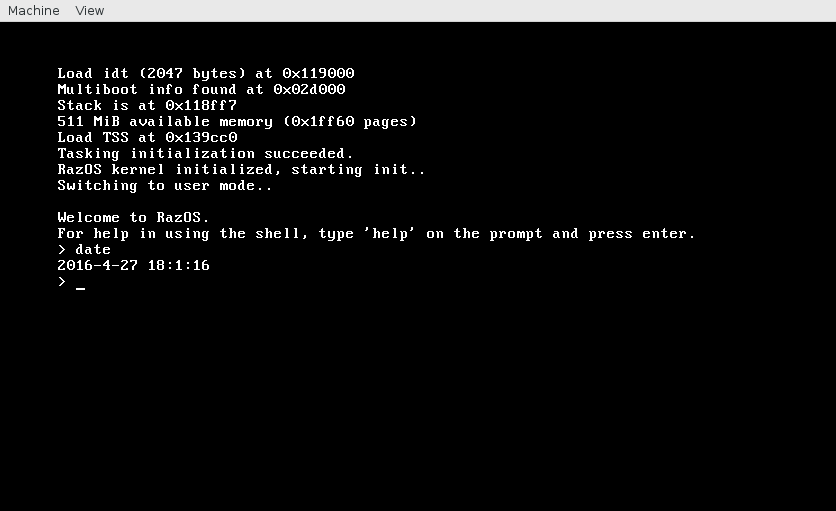
\includegraphics[]{../figures/rash.png}
\label{fig:rash.png}
\end{figure}

\section{Standardityökalut (stdlib.h)}

C-kirjasto stdlib.h määrittelee erilaisia yleishyödyllisiä funktioita, tyyppejä ja makroja, tärkeimpinä dynaamiseen muistinvaraukseen käytettävä malloc, ympäristömuuttujan hallitsemiseen käytettävät getenv- ja setenv-funktiot sekä satunnaislukujen luomiseen käytettävä rand-funktio.

\subsection{Dynaaminen muistinvaraus (malloc)}

Dynaaminen muistinvaraus toimii RazOS:issa hyvin samalla tavoin niin ytimessä kuin käyttäjätilassakin. Käyttäjätilassa jokaisella ohjelmalla on kuitenkin oma virtuaalimuistiavaruus, jossa muistia hallitaan. Koska käyttäjätilalla ei myöskään ole oikeutta käyttää järjestelmäresursseja suoraan, varataan varsinaiset muistisivut brk- ja sbrk-järjestelmäkutsujen avulla.

\subsection{Ympäristömuuttuja (environ)}

Ympäristömuuttuja (environment variable, environ) on osoitin, joka osoittaa merkkijonoista muodostuvaan vektoriin. Nämä merkkijonot sisältävät tietoa ohjelman ympäristöstä, kuten esimerkiksi käytössä olevasta komentotulkista. Kun prosessi kopioidaan fork-järjestelmäkutsulla tai ohjelma aloitetaan exec-järjestelmäkutsulla, ympäristömuuttujan arvot säilyvät.

\par

Koska environ-muuttujan merkkijonojen manuaalinen muuttaminen on virhealtista, POSIX-standardiin kuuluu sen muuttamiseen ja noutamiseen käytettävät setenv- ja getenv-funktiot. Ne on toteutettu myös RazOS:issa.

\subsection{Satunnaisluvut (rand)}

C-kirjaston rand-funktio on näennäissatunnaislukugeneraattori, joka pyrkii matemaattisilla operaatioilla luomaan annetusta siemenarvosta mahdollisimman satunnaisen luvun. RazOS:in rand-funktio täyttää yksinkertaisuudestaan huolimatta C99-standardin minimivaatimukset, ja perustuukin standardin ehdotukseen.

\begin{footnotesize}
\begin{minted}[linenos]{C}
#include <stdlib.h>

static unsigned long next = 1; /* For the rand implementation. */

int rand(void)
{
	next = next * 1103515245 + 12345;
	return((unsigned)(next/65536) % 32768);
}

void srand(unsigned int seed)
{
	next = seed;
}
\end{minted}
\end{footnotesize}

\section{Syöte ja tulostus (stdio.h)}

Tärkeimmät syötteeseen ja tulostukseen liittyvät funktiot löytyvät C-kirjastossa stdio-ylätunnisteen alta. Kirjaston toiminta perustuu täysin käyttöjärjestelmäytimen read- ja write-järjestelmäkutsuihin, sillä vain ydin voi hallita tietokoneen laitteistoja, kuten näyttöä ja näppäimistöä. Käyttäjätilan ohjelmat lukevat ja tulostavat muiden mekanismien avulla, joita Unixissa ovat tekstivirrat ja tiedostodeskriptorit. Jokaiseen tiedostodeskriptoriin liittyy tekstivirta, ja toisaalta jokaista tekstivirtaa vastaa tiedostodeskriptori. Myös standardisyöte (stdin) ja -tuloste (stdout) ovat tiedostodeskriptoreja, joten niitä voidaan käsitellä kuten muitakin tiedostoja. Järjestelmän käsittäminen tiedostojen avulla onkin yksi Unixin periaatteellisista kulmakivistä.

\par

Toinen tärkeä osa Unixin syöte- ja tulostustoimintoja on tekstivirtojen uudelleenohjaus (redirection): ohjelman tuloste voidaankin ohjata johonkin tiedostoon tai toisen ohjelman syötteeksi. Samaten syöte voi tulla näppäimistöltä, toiselta ohjelmalta tai tiedostosta. Ohjelman itse ei tarvitse kuin lukea stdin-tiedostodeskriptoria, sillä järjestelmä hoitaa tekstivirtojen uudelleenohjauksen. Tämä monipuolisuus on syy siihen, miksi Unix käyttää tekstivirtoja yleisenä rajapintana ohjelmien, tiedostojen ja käyttäjien välillä.

\par

RazOS ei syöte- tai tulostustoiminnoiltaan eroa muista POSIX-yhteensopivista Unix-käyttöjärjestelmistä. Käytännön tasolla tekstivirtojen uudelleenohjaus toteutetaan pipe-järjestelmäkutsulla, ja tiedostodeskriptorien luonti vastaavasti dup- ja dup2-järjestelmäkutsuilla. Itse stdio-kirjasto vastaa myös toteutetuilta osin POSIX-standardia, sisältäen esimerkiksi printf-funktion eri muunnelmat.

\section{Komentotulkki}

Komentotulkki on yksi tärkeimmistä ohjelmista Unix-käyttöjärjestelmässä. Se vastaa ohjelmien käynnistämisestä ja prosessinhallinnasta, tekstivirtojen uudelleenohjaamisesta sekä automaatiosta. RazOS:in komentotulkki, Rash, tukee Shell-ohjelmointia lukuun ottamatta näitä komentotulkin perustoimintoja. Erikoisasemastaan huolimatta komentotulkki on Unixissa, kuten RazOS:issakin, vain ohjelma muiden joukossa, eikä sen tiiviimpi osa käyttöjärjestelmää kuin mikään muukaan ohjelma.

\par

Korkealla tasolla komentotulkin toimintaperiaate on varsin yksinkertainen, josta osoituksena alla oleva Rashin syöte-tuloste -silmukka:

\begin{footnotesize}
\begin{minted}[linenos]{C}
static void rash_loop(void)
{
    char *line;
    char **args;
    int status;
    int args_len;
    int i;

    do
    {
        printf("> ");
        line = rash_read_line();
        args = rash_split_line(line, &args_len);
        status = rash_execute(args);

        free(line);
        for (i = 0; i < args_len; i++)
            free(args[i]);
        free(args);
    } while (status);
}
\end{minted}
\end{footnotesize}

Komentotulkin kehitystyö tehtiin GNU/Linux-ympäristössä, josta se siirrettiin pienin muutoksin osaksi RazOS:ia.

\section{Esimerkki standardinmukaisuudesta}

Alla on pieni C-ohjelma, joka tulostaa näytölle päivämäärän ja kellonajan.

\begin{footnotesize}
\begin{minted}[linenos]{C}
#include <stdio.h>
#include <time.h>

int main(void)
{
	time_t t = time(NULL);
	struct tm tm_now = *gmtime(&t);

	printf("%d-%d-%d %d:%d:%d\n",
			tm_now.tm_year + 1900,
			tm_now.tm_mon + 1,
			tm_now.tm_mday,
			tm_now.tm_hour,
			tm_now.tm_min,
			tm_now.tm_sec);
	return 0;
}
\end{minted}
\end{footnotesize}

Ohjelma toimii ilman muutoksia niin RazOS:issa, muissa Unixeissa kuin kaikissa C99-standardin ohjelmointikirjastot sisältävissä käyttöjärjestelmissä.

\chapter{Yhteenveto}

RazOS:in käytettävyydessä on vielä parannettavaa. Suurin puute on kunnollisen päätteen eli terminaaliemulaattorin puuttuminen. Tämä tekee näyttötulosteen tarkasta hallinnasta käyttäjätilassa vaikeaa. Pääteohjelma on kuitenkin jo olemassa, ja se tullaan käyttöjärjestelmän kehitystyön jatkuessa pian lisäämään osaksi järjestelmää.

\par

Unix tunnetaan ehkä parhaiten komentorivityökaluistaan, kuten komennoista grep, awk ja cat. RazOS:issa ei toistaiseksi ole näitä Unixin tuntomerkkejä, mutta niiden lisääminen osaksi järjestelmää on jo nyt täysin mahdollista. Lisäksi mikä tahansa POSIX-yhteensopiva toteutus näistä ja muista ohjelmista voi suoraan toimia myös RazOS:issa.

\par

Lähdekoodi kokonaisuudessaan löytyy GitHubista, osoiteesta \url{https://github.com/Razbit/razos}. Sieltä löytyy myös ohjeet RazOSin ``asentamiseen'' ja käyttämiseen, tiedostosta README.md. Oikealla tietokoneella käyttämistä emme suosittele. Jos tiedoston \texttt{floppy.img} laittaa johonkin emulaattoriin, kuten Qemuun, levykkeeksi, voi käyttöjärjestelmää kokeilla.

\section{Ajankäyttö ja työnjako}

Projekti alkoi jo syksyllä 2014. Sen jälkeen on ollut kaksi täydellistä uudelleenkirjoitusta, ja nykyinen versio sai alkunsa syksyllä 2015. Talven aikana muistinhallinta meni kokonaan uusiksi. Aikaa on siis mennyt todella paljon. GitHubin statistiikat kertovat, että koodia on noin 18000 riviä.

\par

Iiro tuli projektiin mukaan vasta alkusyksystä 2015. Silloin oli kernelin toinen uudelleenkirjoitus alkamassa, ja tehtiin sellainen työnjako, että Iiro tekee käyttäjäpuolta ja Eetu kerneliä. Toki vähän meni ristiin välillä, mutta se oli ajatus ja siinä on melko hyvin pysytty.

\section{Mitä opimme}

Jo ennen projektia meillä oli molemmilla suhteellisen kattava ohjelmointitausta; C oli jo tuttu kieli ja monia ohjelmointiprojekteja oli takana. Tämän kaltainen projekti toi ohjelmointiin aivan uudenlaisen näkökulman: ennen saattoi luottaa siihen, että kirjasto tarjosi kaikenlaisia valmiita funktioita ja tietotyyppejä, mutta käyttöjärjestelmää tehdessä ne on määriteltävä itse. Assymblyllä ohjelmointi oli vierasta, mutta se tuli hyvin tutuksi projektin aikana. Binäärimuotoon käännettyjen ohjelmien rakenteesta saimme valtavan määrän uutta tietoa, kuten myös laitteiston ja ohjelmiston toimimisesta yhdessä. Laitteiston läheinen ohjelmointi oli uutta siinä mittakaavassa, jossa sitä piti käyttöjärjestelmän alimpia osia tehdessä harjoittaa.

\par

Lopputulos, RazOSin toiminnalisuus kirjoitushetkellä, yllätti tekijänsäkin; se toimii yllättävän hyvin, vaikka monesti on meinannut usko loppua. Tekemistä vielä toki on, että pääsisimme tavoitteeseemme: käyttöjärjestelmään, jolla voisi jatkaa sen itsensä kehitystä.

\par

Mitä tekisimme toisin? Montakin asiaa. RazOS on pyritty pitämään mahdollisimman yksinkertaisena, eikä liialliseen optimointiin ole ryhdytty. Se näkyy esimerkiksi siinä, että muistinhallinta on melko hidas, ja heap-alueet fragmentoituvat helposti. Nämä asiat tosin ovat omalla tavallaan projektin tarkoituksen ulkopuolella; nykyiset algoritmit selittävät verrattain yksinkertaisesti käyttöjärjestelmän toimintaa. Ehkä suurin muutos, mikä tulisi tehdä, on virtuaalisen tiedostojärjestelmän toteutus siten, että se tukisi kansioita.


%----------------------------------------------------------------------------------------
%	THESIS CONTENT - APPENDICES
%----------------------------------------------------------------------------------------

\begin{appendices}
\renewcommand\appendixname{Liite}
\appendix % Cue to tell LaTeX that the following "chapters" are Appendices

% Include the appendices of the thesis as separate files from the Appendices folder
% Uncomment the lines as you write the Appendices

\chapter{RazOSin järjestelmäkutsut}

\label{Syscalls}

RazOSissa on kirjoitushetkellä 18 järjestelmäkutsua. Ne on määritelty tiedostossa \texttt{razos/razos\_kernel\_headers/api/razos.h}.

\textbf{sys\_exit}\\
Numero: 0\\
Kutsuminen: \texttt{void exit(int status)}\\
Implementaatio: \texttt{razos/kernel/src/syscall/sys\_tasking.c}\\
Kuvaus: lopettaa prosessin

\textbf{sys\_sched\_yield}\\
Numero: 1\\
Kutsuminen: \texttt{void sched\_yield(void)}\\
Implementaatio: \texttt{razos/kernel/src/syscall/sys\_tasking.c}\\
Kuvaus: luovuttaa suoritusvuoron

\textbf{sys\_fork}\\
Numero: 2\\
Kutsuminen: \texttt{pid\_t fork(void)}\\
Implementaatio: \texttt{razos/kernel/src/syscall/sys\_tasking.c}\\
Kuvaus: jakaa prosessin kahteen samanlaiseen

\textbf{sys\_wait}\\
Numero: 3\\
Kutsuminen: \texttt{uint32\_t wait(int* stat\_loc)}\\
Implementaatio: \texttt{razos/kernel/src/syscall/sys\_tasking.c}\\
Kuvaus: asettaa vanhemman odottamaan lapsiprosessin valmistumista

\textbf{sys\_read}\\
Numero: 4\\
Kutsuminen: \texttt{ssize\_t read(int fd, void* buf, size\_t size)}\\
Implementaatio: \texttt{razos/kernel/src/syscall/sys\_fs.c}\\
Kuvaus: lukee tiedostosta

\textbf{sys\_write}\\
Numero: 5\\
Kutsuminen: \texttt{ssize\_t write(int fd, const void* buf, size\_t size)}\\
Implementaatio: \texttt{razos/kernel/src/syscall/sys\_fs.c}\\
Kuvaus: kirjoittaa tiedostoon

\textbf{sys\_open}\\
Numero: 6\\
Kutsuminen: \texttt{int open(const char* name, int oflag, ...)}\\
Implementaatio: \texttt{razos/kernel/src/syscall/sys\_fs.c}\\
Kuvaus: avaa tiedoston

\textbf{sys\_close}\\
Numero: 7\\
Kutsuminen: \texttt{int close(int fd)}\\
Implementaatio: \texttt{razos/kernel/src/syscall/sys\_fs.c}\\
Kuvaus: sulkee avoimen tiedoston

\textbf{sys\_creat}\\
Numero: 8\\
Kutsuminen: \texttt{int creat(const char* name, mode\_t mode)}\\
Implementaatio: \texttt{razos/kernel/src/syscall/sys\_fs.c}\\
Kuvaus: luo uuden tiedoston

\textbf{sys\_lseek}\\
Numero: 9\\
Kutsuminen: \texttt{off\_t lseek(int fd, off\_t offset, int whence)}\\
Implementaatio: \texttt{razos/kernel/src/syscall/sys\_fs.c}\\
Kuvaus: siirtyy tiedostossa \textit{offset} tavua

\textbf{sys\_fcntl}\\
Numero: 10\\
Kutsuminen: \texttt{int fcntl(int fd, int cmd, ...)}\\
Implementaatio: \texttt{razos/kernel/src/syscall/sys\_fs.c}\\
Kuvaus: hakee tai asettaa monia tiedoston asetuksia/tietoja

\textbf{sys\_fstat}\\
Numero: 11\\
Kutsuminen: \texttt{int fstat(int fd, struct stat* buf)}\\
Implementaatio: \texttt{razos/kernel/src/syscall/sys\_fs.c}\\
Kuvaus: hakee tiedoston status-tietoja

\textbf{sys\_setup}\\
Numero: 12\\
Kutsuminen: \texttt{}\\
Implementaatio: \texttt{razos/kernel/src/syscall/sys\_setup.c}\\
Kuvaus: asettaa tai hakee kernelin asetuksia

\textbf{sys\_pipe}\\
Numero: 13\\
Kutsuminen: \texttt{int pipe(int fd[2])}\\
Implementaatio: \texttt{razos/kernel/src/syscall/sys\_pipe.c}\\
Kuvaus: luo pipen

\textbf{sys\_brk}\\
Numero: 14\\
Kutsuminen: \texttt{int brk(void* addr)}\\
Implementaatio: \texttt{razos/kernel/src/syscall/sys\_uvm.c}\\
Kuvaus: asettaa käyttäjän heap-alueen lopun osoitteeseen \textit{addr}

\textbf{sys\_sbrk}\\
Numero: 15\\
Kutsuminen: \texttt{void* sbrk(intptr\_t incr)}\\
Implementaatio: \texttt{razos/kernel/src/syscall/sys\_uvm.c}\\
Kuvaus: kasvattaa tai pienetää käyttäjän heap-aluetta \textit{incr} tavun verran

\textbf{sys\_execve}\\
Numero: 16\\
Kutsuminen: \texttt{int execve(const char* path, char* const argv[], char* const envp[])}\\
Implementaatio: \texttt{razos/kernel/src/syscall/sys\_execve.c}\\
Kuvaus: vaihtaa suoritettavan ohjelman

\textbf{sys\_time}\\
Numero: 17\\
Kutsuminen: \texttt{time\_t time(time\_t* timer)}\\
Implementaatio: \texttt{razos/kernel/src/syscall/sys\_time.c}\\
Kuvaus: palauttaa ajan sekunteina UNIXin Epochista, 1.1.1970 UTC00:00:00


\end{appendices}
%----------------------------------------------------------------------------------------
%	BIBLIOGRAPHY
%----------------------------------------------------------------------------------------

\nocite{*}
\printbibliography[title={Kirjallisuus ja lähteet}, heading=bibintoc]

%----------------------------------------------------------------------------------------

\end{document}
